\documentclass{article}

\usepackage[normalem]{ulem}
\usepackage{fancyhdr}
\usepackage[parfill]{parskip}
\usepackage{tikz}
\usepackage{pgfplots}
\usepackage{multicol}
\usepackage[version=3]{mhchem}
\usepackage{SIunits}
\usepackage{lscape}
\usepackage{array}
\usepackage{hyperref}
\usepackage{bookmark}
\makeatletter
\renewcommand\@seccntformat[1]{}
\makeatother

\newcolumntype{x}[1]{%
>{\centering\arraybackslash}m{#1}}

\pagestyle{fancyplain}

\pgfplotsset{compat=1.7}

\title{15 - X-rays}
\author{Todd Davies}
\date{\today}

\begin{document}

\rhead{15 - X-rays}
\lhead{\today}

\maketitle

\section{Production of X-rays}
\thispagestyle{empty}

X-rays are a form of electromagnetic radiation, and have a wavelength of between
$10^{-8}m$ and $10^{-13}m$. They behave in a very simimlar way to gamma rays,
the only real difference is how they are produced:

{\bf X-rays} are produced when fast moving electrons are rapidly
decelerated. As the electrons slow down, their kinetic energy is transformed
into photons of electromagnetic radiation.

{\bf Gamma rays} are produced by radioactive decay. Gamma photons are
usually produced after an alpha or Beta emmision.

X-rays used in medical applications are often described as {\it soft} since they
generally have lower energies (so patients don't get too ionised).

\subsection{X-ray tubes}

X-ray tubes produce X-rays in medical applications. They contain a cathode and
an anode inside a vacuume. The cathode is a heated filament that emitts
electrons. The anode is a rotating disk of tungsten.

A potiential difference of around $200\kilo\volt$ is applied to the
anode and cathode so that electrons are accelerated across the space between
them. When they hit the anode, they have an energy of $200\kilo\electronvolt$
and so have a very high kinetic energy. They lose some of that kinetic energy in
the collision, which is converted into X-rays.

The X-rays are emmited in all directions, but the casing of the tube has a part
that allows the X-rays to escape so that they can be directed onto the patient.

Only about 1\% of the energy of the electrons is converted into X-rays, the
remaining energy is converted into heat, which is why the anode rotates.

\subsection{X-ray spectrum}

The X-rays produced by X-ray tubes can be analyzed plotted on a graph as shown
below:

\begin{center}
	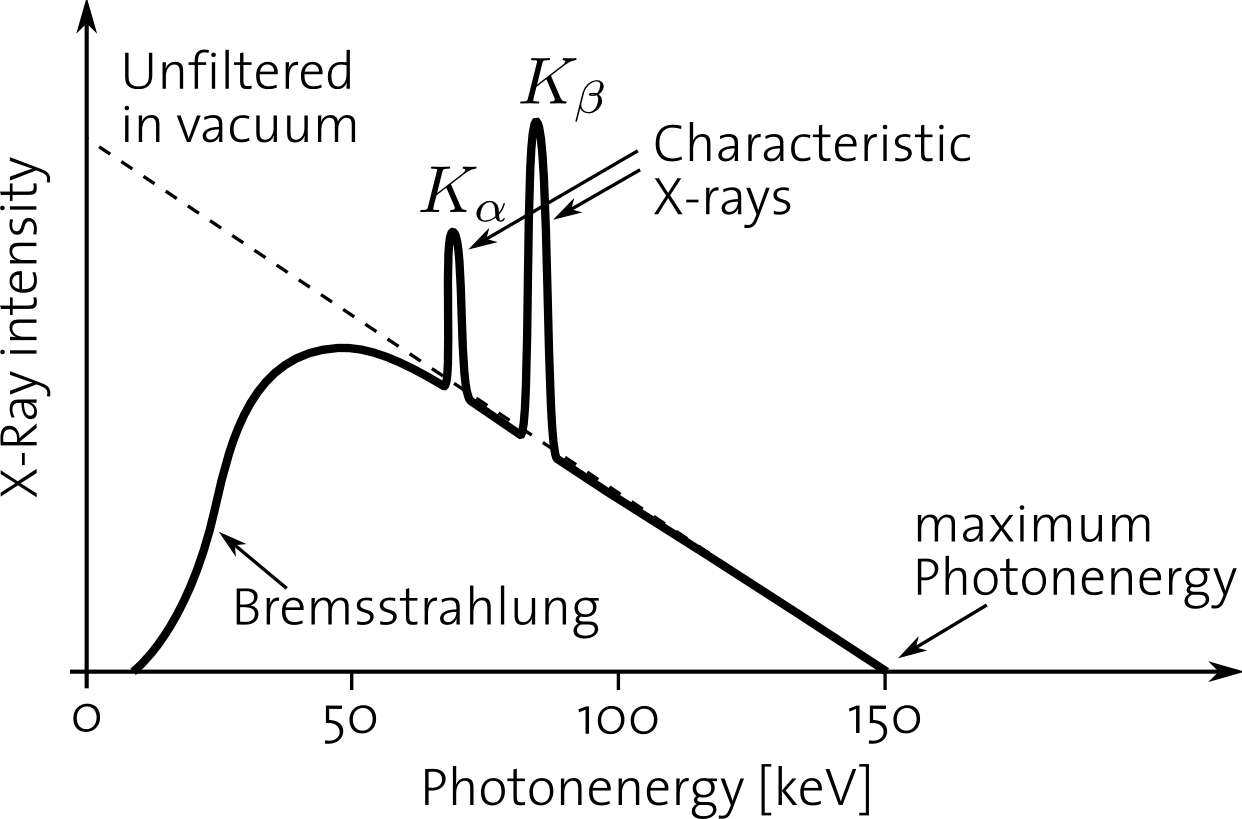
\includegraphics[scale=0.8]{Characteristic_Spectrum}
\end{center}

The Bremsstrahlung radiation (or the 'hump') is formed because not all of the
X-rays produced have identical energies (some electrons lose energy through
interaction with positive nuclei or maybe release different amounts of photons).

The two spikes are X-rays characteristic of the metal used in the anode (usually
tungsten, but sometimes copper or molybednum). They represent the energies
between energy levels in the atoms that make up the metal (as you will recall
from G482). In practice, these are unimportant in medical applications.

\section{X-ray attenuation}

Intensity is defined as the power per unit cross-sectional area. The intensity
of a collimated \marginpar{{\bf Collimated}: All the particles/rays are moving in the
same direction} beam decreases as it passes through matter. This phenomenon is called
attenuation.

The equation that represents the attenuation of an X-ray as it passes through a
uniform material is:

\[
	I = I_0e^{-\mu x}
\]

Where:

\begin{center}
	\begin{tabular}{|l|l|}
		\hline
		{\bf Symbol} & {\bf Quantity} \\ \hline
		$I$ & Final intensity \\ \hline
		$I_0$ & Initial intensity \\ \hline
		$\mu$ & The coefficient of attenuation \\ \hline
		$x$ & The thickness of the material \\ \hline
	\end{tabular}
\end{center}

Elements with a higher atomic number (in general) are able to attenuate X-rays
more strongly.

Since different materials have different coefficients of attenuation, the
internal composition of objects can be determined by measuring the intensity of
X-rays that have passed through them. This is (in a sense) how X-ray machines
work. The atoms inside bones have a higher atomic number than those found in
flesh and so attenuate X-rays more strongly. Henceforth, the X-rays passing out
of the bones are of a lower intensity.

\subsection{Absorbsion mechanisms}

There are three mechanisms by which X-rays can be absorbed by atoms. They are
described on the next page.

\begin{landscape}
\begin{table}
\centering
\def\arraystretch{1.5}
\begin{tabular}{|x{2cm}|x{3cm}|x{5cm}|x{3cm}|x{3cm}|}

	\hline
	
	{\bf Attenuation mechanism} & 
	{\bf Energy range of incoming X-ray photons} & 
	{\bf What happens to the X-ray photon} & 
	{\bf Relationship between $\mu$ and $Z$} & 
	{\bf Relationship between $\mu$ and $E$} \\ \hline

	Photoelectric effect & $<0.1MeV$ & Photon disappears and removes an electron from the atom. & $\mu \propto Z^3$ & $\mu \propto \frac{1}{E^3}$ \\ \hline

	Compton scattering & $0.5-5.0MeV$ & Photon is inelastically scattered by atomic electron. The scattered photon has a lower energy. & $\mu$ is independent of $Z$ & Decreases slowly with $E$ \\ \hline

	Pair production & $>1.02MeV$ & Photon dissapears and produces an electron positron pair. & $\mu \propto Z^2$ & Rises slowly with $E$ \\ \hline

\end{tabular}

\end{table}
\end{landscape}

Here are diagrams of the three:

{\bf Photoelectric effect}

\begin{center}
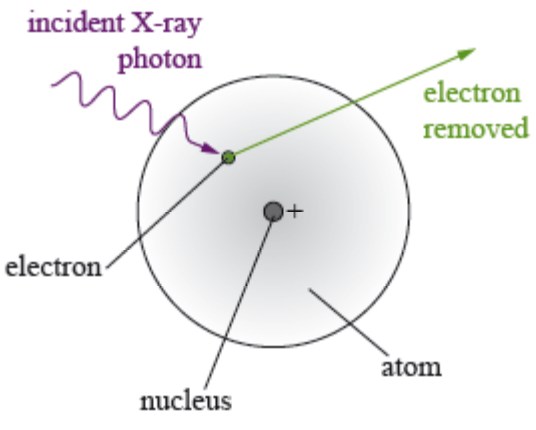
\includegraphics[scale=0.3]{photoelectric}
\end{center}

{\bf Compton scattering}

\begin{center}
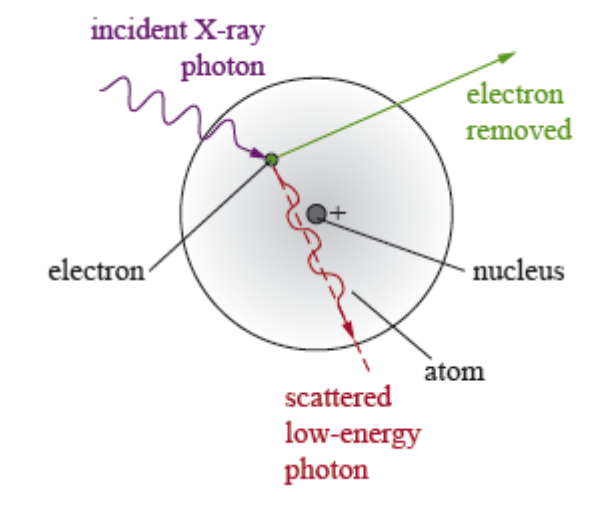
\includegraphics[scale=0.3]{compton}
\end{center}

{\bf Pair production}

\begin{center}
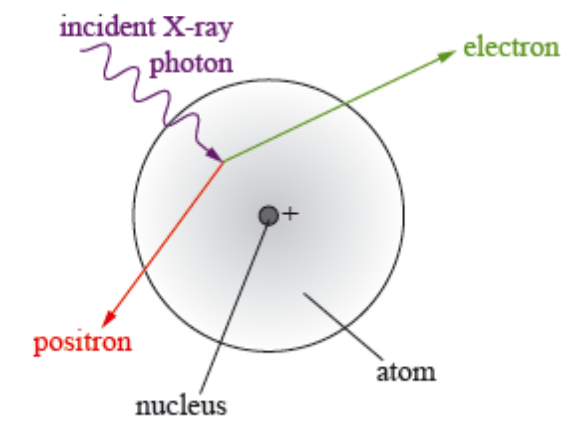
\includegraphics[scale=0.3]{pair_production}
\end{center}

\section{Improving X-ray images}

It is desirable to be able to obtain high quality images from X-rays, since it
maximises the amount detail shown in the image. Not only are bones visible, but
soft tissue such as organs and blood vessels. Radiographers also want to make
sure that the patient's exposure to radiation is minimal so that the risk of
cancer and other side effects is minimised.

X-rays can be detected by film or by digital sensors. Traditional film is not
very sensitive to X-rays, so intensifier screens are used to increase the
contrast.

An intensifier screen contains a phosphor that fluoresces when it absorbs X-ray
photons. Each X-ray photon that hits the intensifier emmits thousands of visible
photons, which reduces the patient's exposure by around 500\%.

Digital systems work in much the same way, except that a CCD (charge coupled
device) is used to image the light photons produced by the intensifier screen.

\subsection{Improving contrast}

A contrast medium is a substance that a patient can swallow or have injected
into them that absobs X-rays. It allows the outlines of soft tissue to be imaged
using an X-ray machine. Contrast media have a high atomic number and readily
absorb X-rays, mainly by the photoelectric effect.

\subsection{Computerised axial tomography}

A CAT(computeried axial tomography) scan shows a patient in three dimensions, as
opposed to an X-ray image that is essentially a two dimensional shadow.

In a CAT scan, the patient lies inside a ring of X-ray detectors, while an X-ray
tube rotates around him. The detectors opposite the tube send electronic images
to a computer which then builds up a three dimensional image of the patient.

In later generations of CAT scanners, the patient is moved slowly through the
ring of detectors so that the whole body (or an arbitary portion of the body)
can be imaged.

CAT scans are advantageous since they show three dimensional relationships
between different tissues, and can distinguish between tissues with very similar
attenuation coefficients.

\end{document}